\documentclass[thesis]{poster_style}
\usepackage{graphicx}
\usepackage{natbib}
\usepackage{booktabs}
\usepackage{subfig}
\usepackage{amsmath}
\usepackage{textcomp}
\usepackage{url}
\usepackage{tikz}
\usetikzlibrary{quotes,arrows.meta}
\usepackage[utf8]{inputenc}
\usepackage{amssymb}
\usepackage{caption}
\usepackage{float}
\graphicspath{{Images/}} 
\usepackage{tocbibind}
\usepackage{tabularx}
\usepackage{amsmath}
\usepackage{appendix}
\usepackage{hyperref}
\usepackage{blindtext}
\usepackage{url}
\usepackage{xcolor}
\usepackage{sectsty}

\sectionfont{\color{bordercolor}}
\subsectionfont{\color{bordercolor}}

%% Author of the thesis.
\author{Conor Casey}

%% The year of your thesis poster's creation.
\posteryear{2019}

%% Thesis Title.
\title{AMSIMP: An Open Source Implementation to Simulating \\ Tropospheric and Stratospheric Dynamics \\ on a Synpotic Scale}

%% Teacher name.
\advisor{Ms. Abbott}

%% School name.
\reader{Pobalscoil Inbhear Scéine}

\pagestyle{fancy}

\begin{document}

\begin{poster}

\section{Introduction}
This \textbf{project hypothesises} that it is \textbf{possible to create} an
\textbf{open-source implementation} to \textbf{simulating tropospheric} and
\textbf{stratospheric dynamics} on a \textbf{synoptic scale}, that \textbf{such software}
is \textbf{consistent and reliable}, and that the software \textbf{consists of high-quality source code}.

\section{Parameterisation of Simulation}
Within the software, the \textbf{globe} is \textbf{divided into cells}. You can imagine
this as \textbf{cutting} the \textbf{atmosphere} up into \textbf{cuboids} of air of \textbf{equal volume}.
It then \textbf{solves} the relevant \textbf{equation} at the \textbf{middle} of the
\textbf{cell}. After which point, this value is \textbf{used as} an
\textbf{approximation} for the \textbf{entire cell}. 

\hfill

\begin{center}
    \begin{tikzpicture}[every edge quotes/.append style={auto, text=black}]
        \pgfmathsetmacro{\cubex}{10}
        \pgfmathsetmacro{\cubey}{5}
        \pgfmathsetmacro{\cubez}{7.5}
        \draw [draw=black, every edge/.append style={draw=black, densely dashed, opacity=.5}]
        (0,0,0) coordinate (o) -- ++(-\cubex,0,0) coordinate (a) -- ++(0,-\cubey,0) coordinate (b) edge coordinate [pos=1] (g) ++(0,0,-\cubez)  -- ++(\cubex,0,0) coordinate (c) -- cycle
        (o) -- ++(0,0,-\cubez) coordinate (d) -- ++(0,-\cubey,0) coordinate (e) edge (g) -- (c) -- cycle
        (o) -- (a) -- ++(0,0,-\cubez) coordinate (f) edge (g) -- (d) -- cycle;
        \path [every edge/.append style={draw=black, |-|}]
        (b) +(0,-25pt) coordinate (b1) edge ["$\Delta \lambda$"'] (b1 -| c)
        (b) +(-25pt,0) coordinate (b2) edge ["$\Delta z$"] (b2 |- a)
        (c) +(17.5pt,-17.5pt) coordinate (c2) edge ["$\Delta \phi$"'] ([xshift=17.5pt,yshift=-17.5pt]e);
    \end{tikzpicture}
\end{center}

The \textbf{key equations} utilised within the software are represented
\textbf{in discretized form} below:

\begin{equation}
    u_g = -\frac{1}{\rho f} \frac{\Delta p_y}{2 \Delta y}
    \label{u}
\end{equation}

\begin{equation}
    v_g = \frac{1}{\rho f} \frac{\Delta p_x}{2 \Delta x}
    \label{v}
\end{equation}

\begin{equation}
    T^{n + 1}_{x, y, z} = T^{n - 1}_{x, y, z} + u \frac{\Delta t}{\Delta x} (\Delta T_{x})
    + v \frac{\Delta t}{\Delta y} (\Delta T_{y})
    \label{temp}
\end{equation}

\begin{equation}
    W^{n + 1}_{x, y, z} = W^{n - 1}_{x, y, z} + u \frac{\Delta t}{\Delta x} (\Delta W_{x})
    + v \frac{\Delta t}{\Delta y} (\Delta W_{y})
    \label{pwv}
\end{equation}

\begin{equation}
    \rho^{n + 1}_{x, y, z} = \rho^{n - 1}_{x, y, z} - u \frac{\Delta t}{\Delta x} (\Delta \rho_{x})
    - v \frac{\Delta t}{\Delta y} (\Delta \rho_{y})
    \label{mass_continuity}
\end{equation}

\begin{equation}
    p = \rho R T
    \label{state_eq}
\end{equation}

\section{Contour Plot}

\begin{center}
    \begin{figure}
        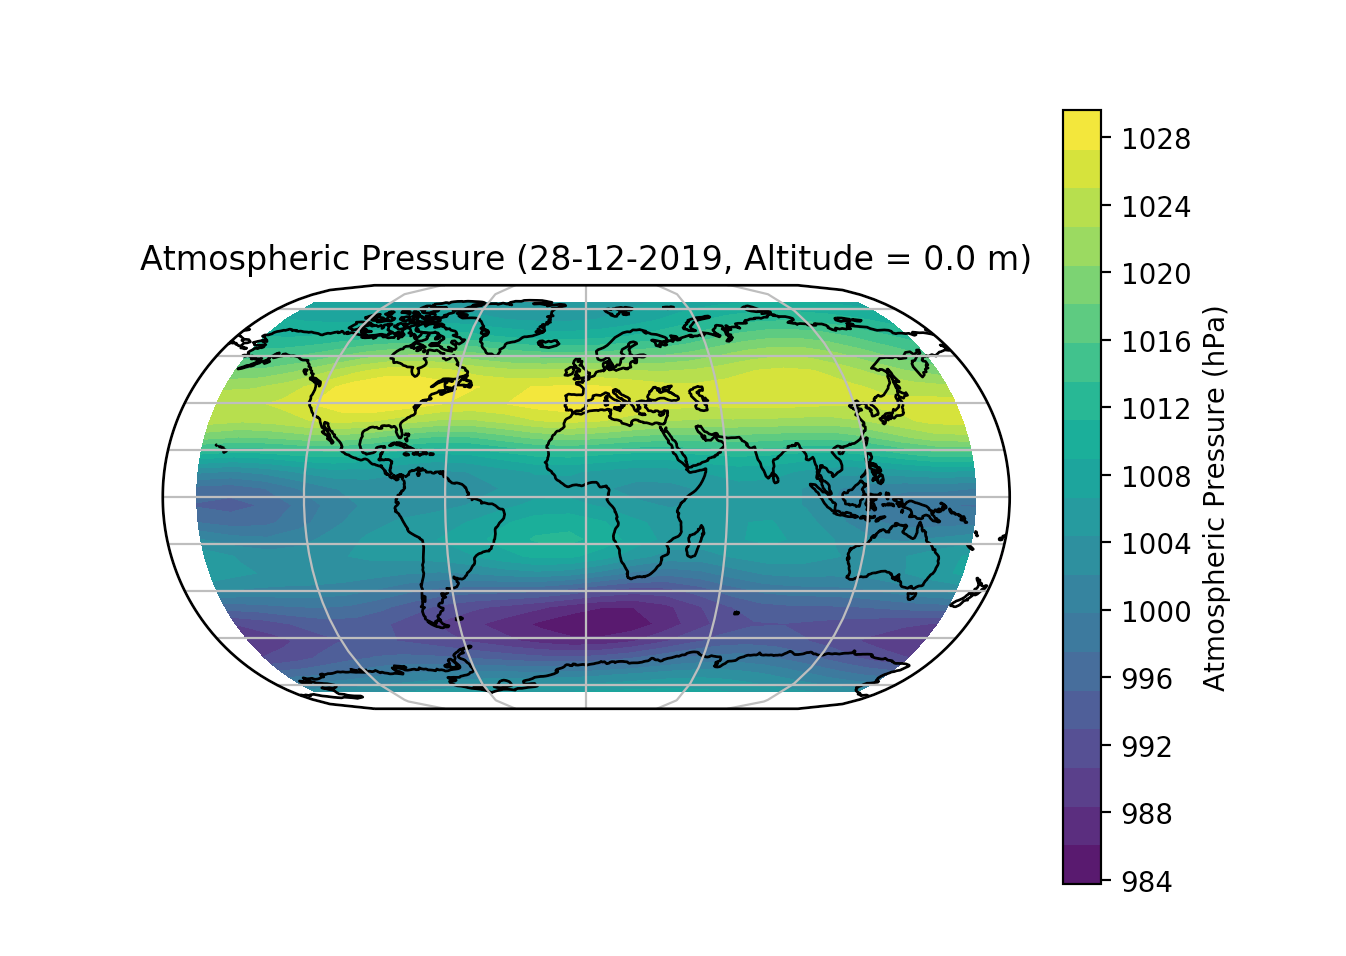
\includegraphics[width=.65\linewidth]{pressure.png}
        \caption{An Example Atmospheric Pressure Contour Plot}
    \end{figure}
\end{center}

\section{Open Source Software}
\textbf{Open Source Software} is software with \textbf{source code}
that \textbf{anyone} can inspect, \textbf{modify}, and enhance. \textbf{Programmers with access}
to the source code can \textbf{improve} that \textbf{program} by
\textbf{adding features} to it, or by \textbf{fixing bugs}. If an \textbf{atmospheric dynamics simulator} 
became \textbf{available} to the \textbf{open source community}, it could
\textbf{lead to} a \textbf{low cost}, and \textbf{high quality simulator} ultimately being
produced. If such an event occurs, it could, \textbf{theoretically},
vastly \textbf{enhance} existing \textbf{numerical weather prediction software}.

\section{Benchmarking Method}%

To prove the hypothesis, it was determined that a series of appropriate
benchmarks would be carried out in the areas of performance, accuracy,
and code quality.

\begin{itemize}
\item The \textbf{performance benchmark} would \textbf{demonstrate whether} 
or not the \textbf{software} has \textbf{consistent and reliable performance}.
\item The \textbf{accuracy benchmark} would \textbf{highlight whether} or not
the \textbf{forecasts produced} by the software has a \textbf{reasonable level of accuracy}.
\item The \textbf{code quality benchmark} would \textbf{indicate whether} or not the \textbf{source code} 
of the software was \textbf{of high quality}.
\end{itemize}

\section{Results}%

\begin{center}
\begin{tabular}{|c|c|c|c|} 
 \hline
 Forecast Day & $\bar{x}$ & $\sigma$ & $\frac{\sigma}{\bar{x}}$ \\
 \hline
 1 & 48.71941 & 1.6192 & 0.03324 \\
 \hline
 2 & 82.05565 & 3.14003 & 0.03827 \\
 \hline
 3 & 122.0275 & 6.96494 & 0.05708 \\
 \hline
 4 & 164.84392 & 6.02163 & 0.03653 \\
 \hline
 5 & 209.37133 & 7.62972 & 0.03644 \\
 \hline
\end{tabular}\par
\end{center}

In regards to the performance benchmark, the time it took to generate a five-day forecast was measured. The
\textbf{statistical analysis} of the results \textbf{found} that the \textbf{mean coefficient of variation} 
($\frac{\sigma}{\bar{x}}$) was approximately, \textbf{0.04}.

\begin{center}
    \begin{figure}
        \includegraphics[width=.5\linewidth]{mape_graph.png}
        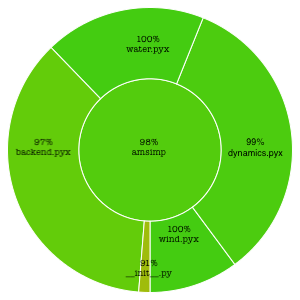
\includegraphics[width=.36\linewidth]{code_coverage.png}
        \caption{Results of Accuracy (L) and Code Quality (R) Benchmarks}
    \end{figure}
\end{center}

In regards to the accuracy benchmark, it showed that a \textbf{four-day forecast}
produced software had a \textbf{mean absolute percentage error}
of approximately \textbf{1.56\%}.

In regards to the code quality benchmark, it indicated
that the software had a \textbf{code coverage} of approximately \textbf{98\%}.

\section{Conclusions}
The results of the \textbf{performance benchmark demonstrated} that there was a \textbf{low variation} 
in \textbf{execution time}, proving that the \textbf{performance of the software}
was \textbf{consistent and reliable}. The results of the \textbf{accuracy benchmark indicated}
that the \textbf{forecast produced} by the software is \textbf{accurate}, which further proves its consistency and reliability. This \textbf{code quality benchmark signified}
that the \textbf{software has} a \textbf{lower chance} of \textbf{containing undetected bugs}, ultimately
\textbf{demonstrating} that the \textbf{quality of} the \textbf{source code is high}.

\end{poster}

\end{document}

 
